

\section{Results}
\label{sec:results}

% TODO: co-author to write the results section here.
[Results go here, written after data collection.
Suggested subsections: participants, session-level summaries,
questionnaire outcomes.]

% ,,,,,,,,,,,,,,,,,,,,,,
\subsection{Example session}
\label{sec:example-session}
% ,,,,,,,,,,,,,,,,,,,,,,

Figure~\ref{fig:session-overview} follows one recorded session in
the acrophobia scenario from calibration to the end of the run.
Over the 312~s run the system sent 98 \texttt{increase} and 123
\texttt{decrease} commands, and the balloon rose and fell twice
within a range of 15 to 80~m. The session illustrates the loop in
operation and is not intended as a summary of the recorded set.

\begin{figure}[H]
    \centering
    \IfFileExists{diagrams/07-session-overview.png}{%
        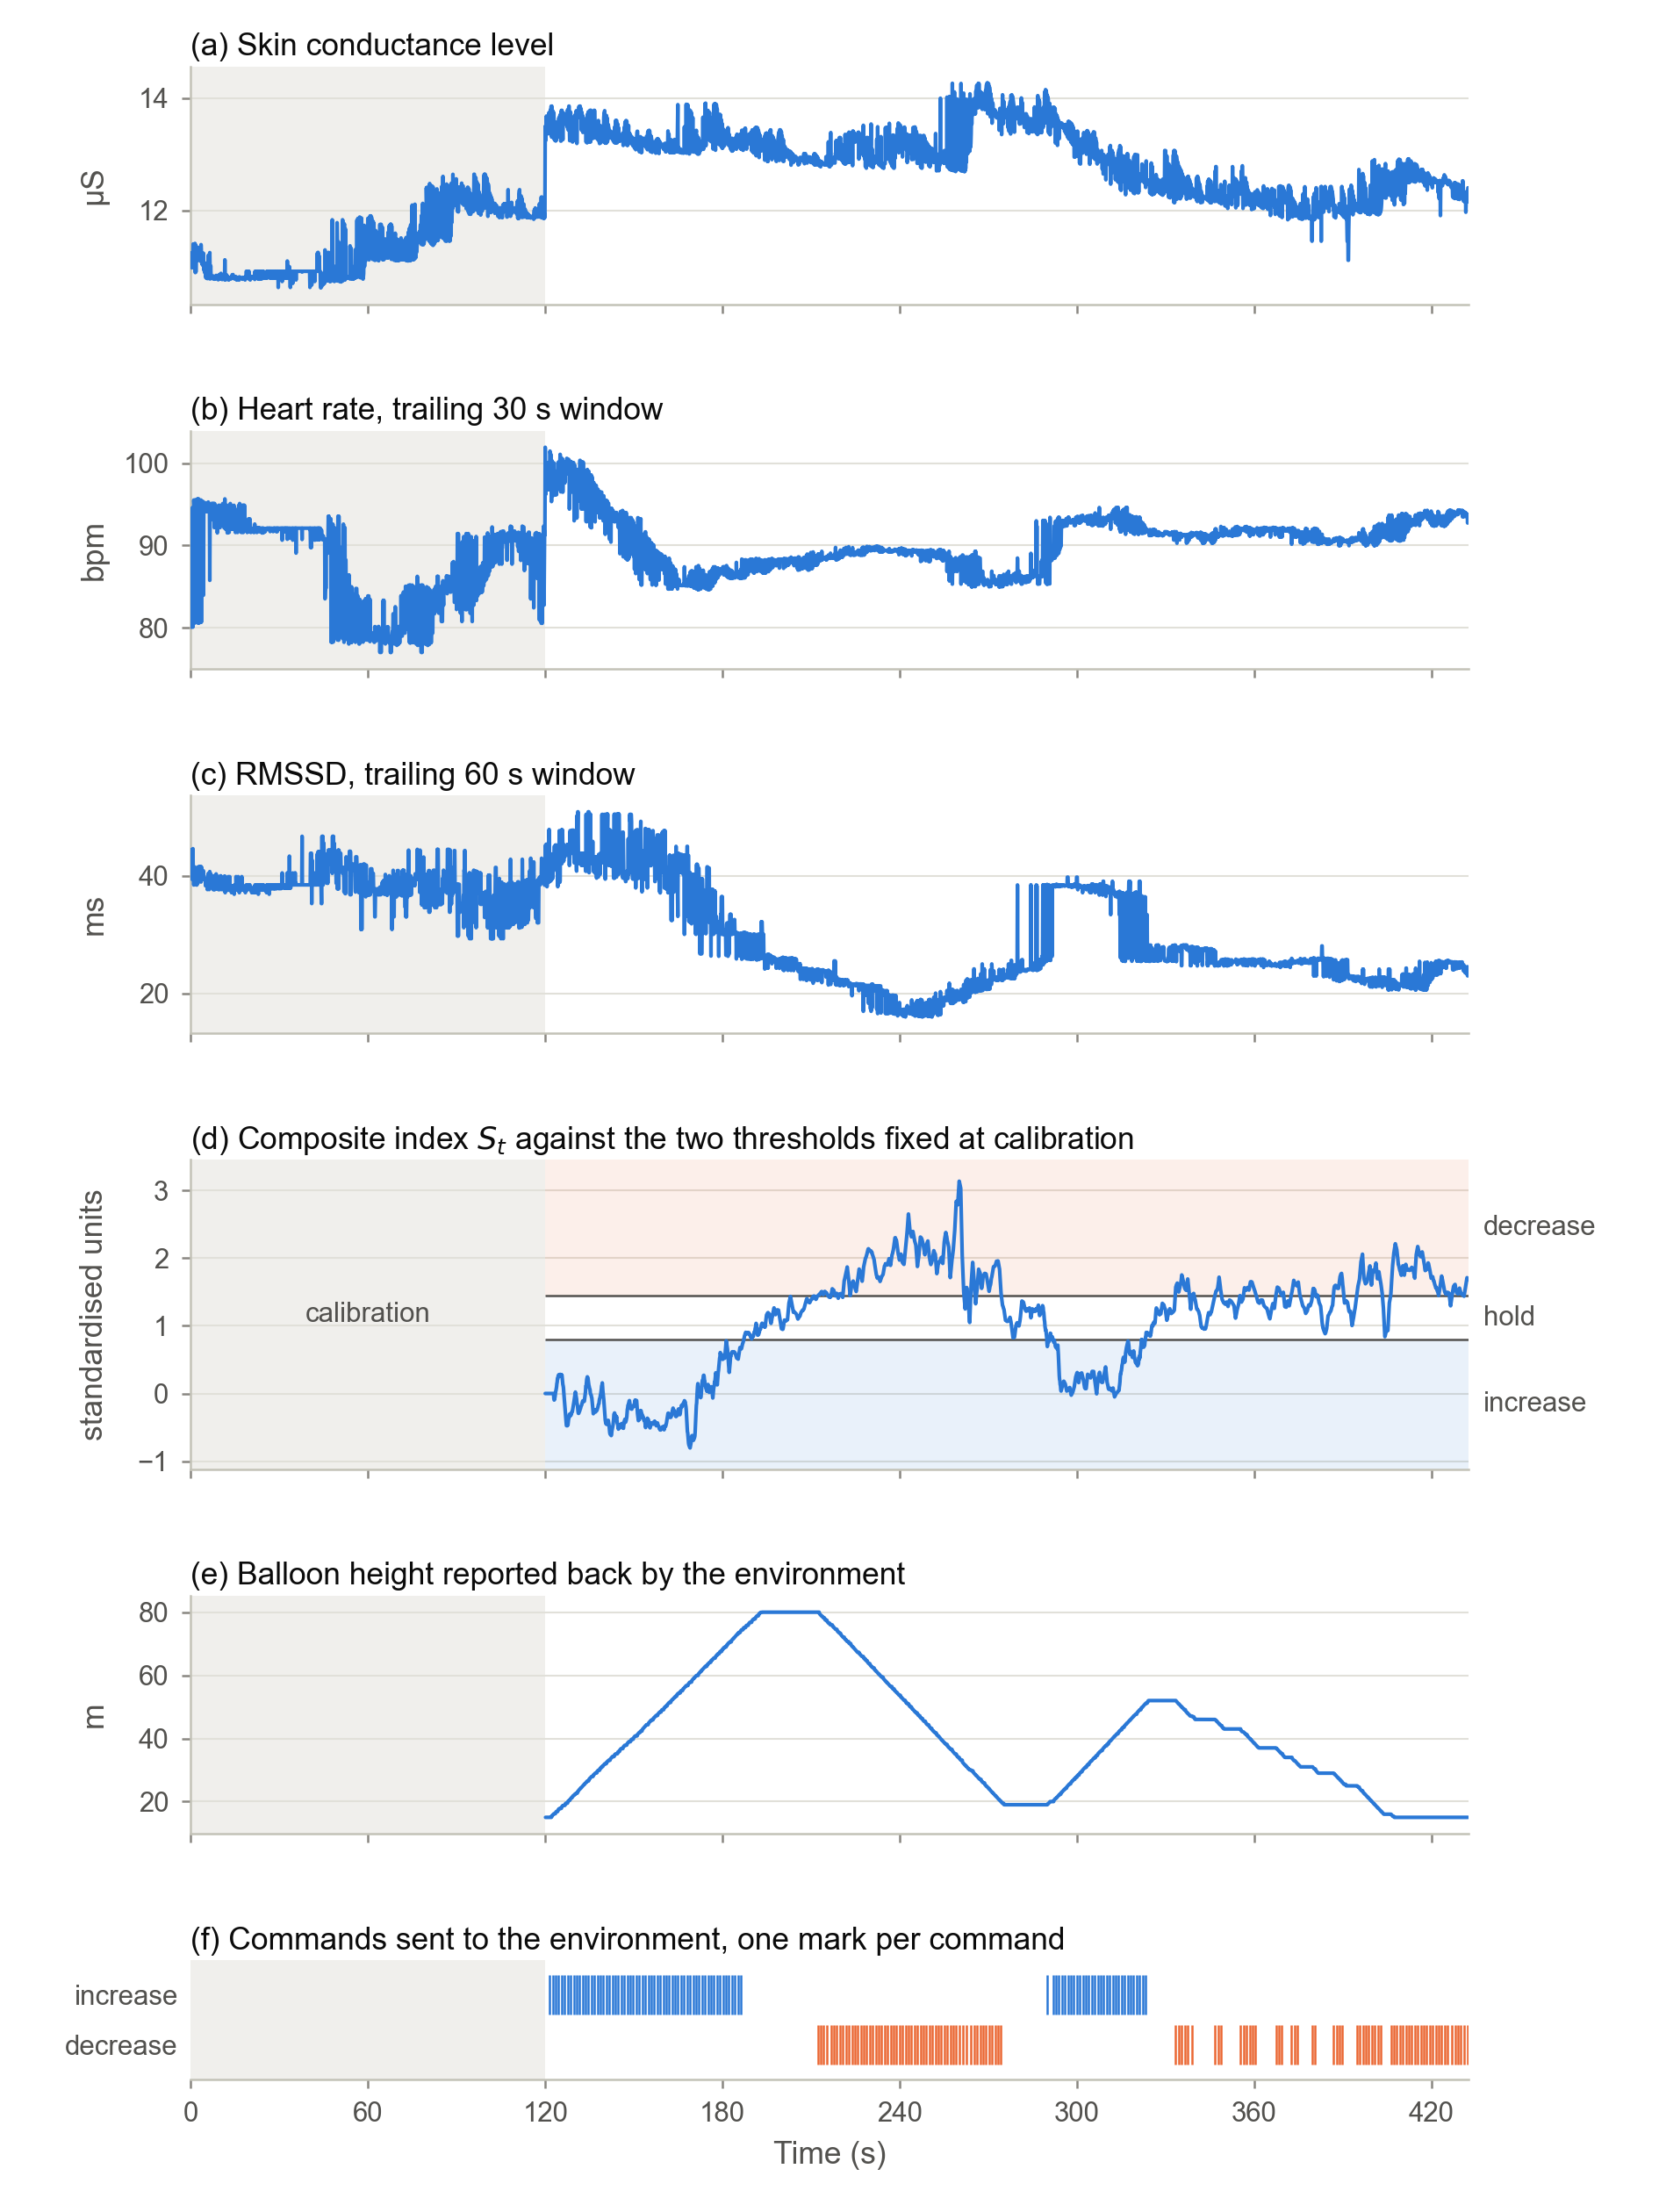
\includegraphics[width=\linewidth, height=0.9\textheight, keepaspectratio]{diagrams/07-session-overview.png}%
    }{%
        \fbox{\parbox{0.9\linewidth}{\centering
            \vspace{1.5cm}
            \textbf{[Figure placeholder, session overview]}\\[6pt]
            \small Place the exported image in \texttt{diagrams/}.
            \vspace{1.5cm}
        }}%
    }
    \caption{One recorded session in the acrophobia scenario. The
    two thresholds were fixed at the end of the 120~s calibration
    (shaded). While the composite index stays below the lower
    threshold the system sends \texttt{increase}, above the upper
    threshold it sends \texttt{decrease}, and between the two it
    sends nothing; the balloon height reported by the environment
    follows. The pause between calibration and the start of the run
    is not recorded and is omitted from the time axis.}
    \label{fig:session-overview}
\end{figure}

% ,,,,,,,,,,,,,,,,,,,,,,
\subsection{Extraction backend agreement}
\label{sec:results-backends}
% ,,,,,,,,,,,,,,,,,,,,,,

Table~\ref{tab:backend-agreement} and
Figure~\ref{fig:backend-comparison} report the comparison
described in Section~\ref{sec:crossval} over one archived
recording.

\begin{table}[H]
    \centering
    \renewcommand{\arraystretch}{1.4}
    \setlength{\tabcolsep}{9pt}
    \small
    \begin{tabular}{@{}p{3.4cm}p{2.0cm}p{2.2cm}p{2.2cm}p{3.2cm}@{}}
        \toprule
        \textbf{Quantity} &
        \textbf{Pearson $r$} &
        \textbf{RMS diff.} &
        \textbf{Mean diff.} &
        \textbf{Note} \\
        \midrule
        Heart rate &
            \textit{tbd} & \textit{tbd} & \textit{tbd} &
            all valid samples \\
        \addlinespace[5pt]
        RMSSD &
            \textit{tbd} & \textit{tbd} & \textit{tbd} &
            clean segments only \\
        \addlinespace[5pt]
        Composite index &
            \textit{tbd} & \textit{tbd} & \textit{tbd} &
            all valid samples \\
        \bottomrule
    \end{tabular}
    \caption{Agreement between the two extraction backends over a
    single archived recording, computed as described in
    Section~\ref{sec:crossval}.}
    \label{tab:backend-agreement}
\end{table}

\begin{figure}[H]
    \centering
    \IfFileExists{diagrams/06_backend_comparison.png}{%
        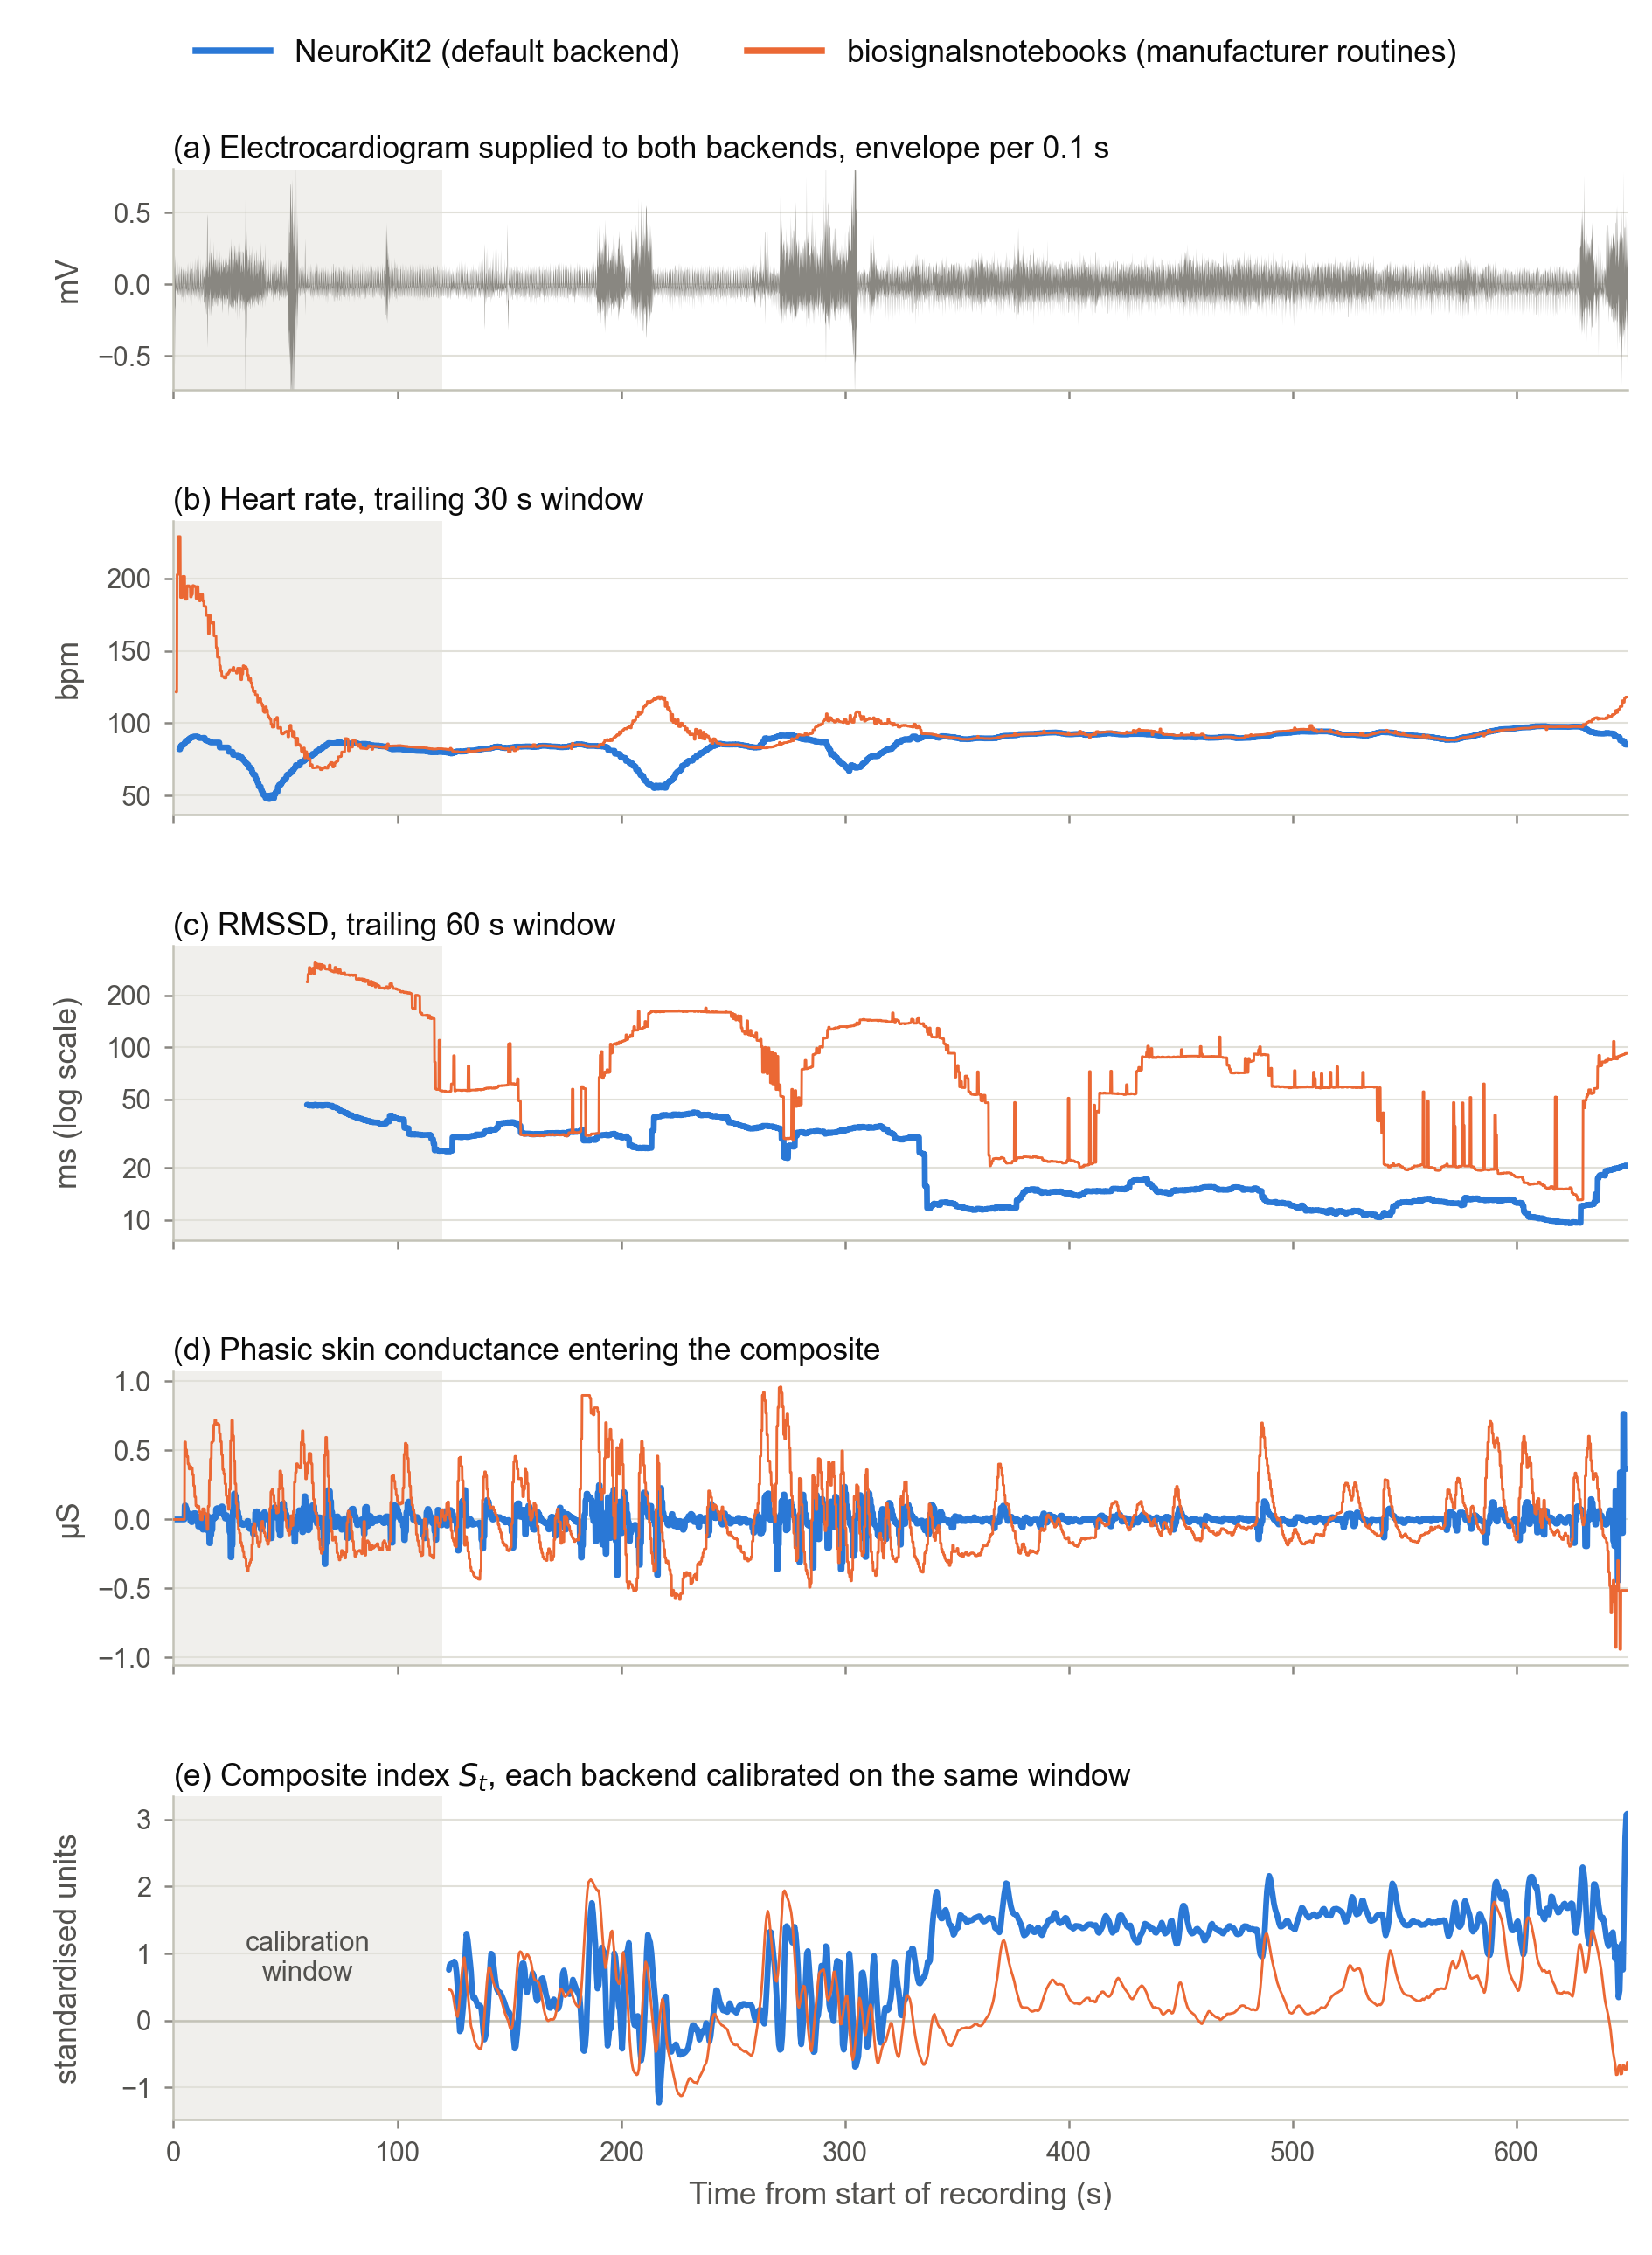
\includegraphics[width=\linewidth, height=0.9\textheight, keepaspectratio]{diagrams/06_backend_comparison.png}%
    }{%
        \fbox{\parbox{0.9\linewidth}{\centering
            \vspace{1.5cm}
            \textbf{[Figure placeholder, backend comparison]}\\[6pt]
            \small Produced by the comparison script from a raw
            capture file. Place the exported image in
            \texttt{diagrams/}.
            \vspace{1.5cm}
        }}%
    }
    \caption{Both extraction backends driven over one archived
    recording of 649~s captured at 1000~Hz. From the top: the
    electrocardiogram supplied to both, heart rate, RMSSD on a
    logarithmic axis, the phasic conductance entering the composite,
    and the composite index, with each backend calibrated on the
    same first 120~s (shaded). Divergence is attributable to
    extraction alone, the input being identical.}
    \label{fig:backend-comparison}
\end{figure}

[Interpretation of the agreement values, written once they are
regenerated for the current version of the code.]
